\documentclass[11pt]{article}

% the percent sign gives comments in Latex
% top line indicates this is for Physical Review, standard journal format,
% suitable for electronic submission of articles

% the line above is necessary to start any latex document.
% this is one variation that should work for most things.
% if you want double spaceing, use the following:
%
%\documentclass[prd,preprint,letterpaper]{revtex4}
%
% the "preprint" designation will make a wider line
% spacing, good for markup.
\usepackage{graphicx}  % this is the up-to-date package for all figures
\usepackage{float}	% allows use of 'H' command

% these are some custom control of the page size and margins
% \topmargin= 0.2in  % these 1st two may be needed for some computers
%\textheight=8.75in
\textwidth=6.5in
\oddsidemargin=0cm
\evensidemargin=0cm

% this is where the actual document itself (rather than control statements) begins:

\begin{document}

% use a style that gives automatic headings
\pagestyle{myheadings}

% the \title{} command generates a title.

% the \\ below is used to FORCE a line break in the middle of the sentence--
% otherwise latex computes it for you

\title{Lab 5:\\
Monte-Carlo Integration}


\author{Corey Mutnik \\
{\it Computational Physics 305, University of Hawaii at Manoa} }


\date{February 17, 2015}




\maketitle    % this line is necessary to tell latex you are done with all
	      % of the stuff associated with the title, and now it can go
              % ahead and generate the title portion


	      % \section is used to start a new one with a heading
\abstract{

The Monte-Carlo method of integration allows us to calculate amount of space something occupies knowing nothing 
more than its boundaries.  In the simple case of estimating the area of a cicle/sphere inscribed in a square/cube 
we used a hit ratio to estimate the amount of space each object occupied (area/volume).  This simple notion can 
than be applied to objects with higher dimensionality.  By knowing the equations governing an objects boundaries 
and calculating its hit ratio we are able to estimate the "volume" of such an object, independent of what dimension 
it resides in.

}

\section{Introduction}

The total number of trial minutes recorded in the data set, N, is know.  This allows us to use the normalized 
P
\begin{equation}
\label{1}
V_{unknown}=\frac{N_{hit}}{N_{tot}}V_{tot}
\end{equation}



% one or more lines of space between paragraphs determines them
\section{Code}

Various programs and plot files can be seen online at: \\
http://www2.hawaii.edu/$\sim$cmutnik/lab6.html


\section{Computational problem}

N is known.  Therefore, the fit overlapping our data is the normalized Poisson:\\
\begin{equation}
\label{NormalizedP}
P(k~:~ \mu,~N) ~=~ N~ \mu^k \frac{e^{-\mu}}{k!}
\end{equation}

\section{Graphs}

\begin{figure}[H]
  \begin{center}
\centerline{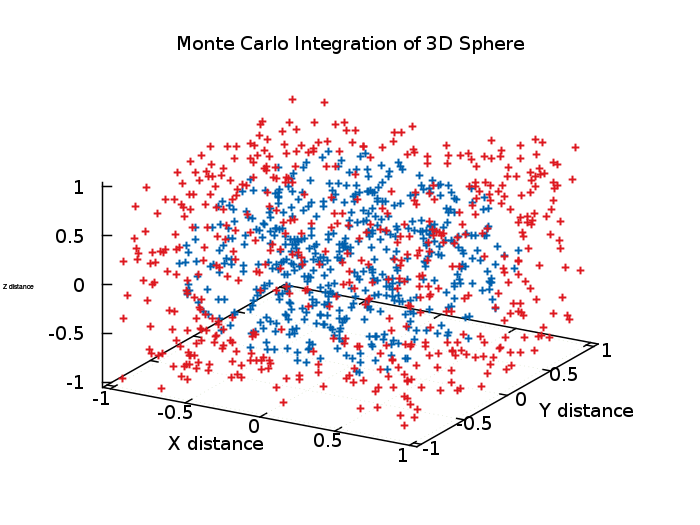
\includegraphics[width=3.75in]{3dvol.png}}
\caption{\it \small{Graphical representation of a Monte Carlo Integration for a 3D sphere \label{fig1}}}
  \end{center}
\end{figure}






\section{Analysis}




\section{Conclusion}





% the following \setlength is to force the bibliography to have no
% paragraph indentations.Can use vairous units--cm are used here.
\setlength{\parindent}{0cm}

\begin{thebibliography}{99}  % the trailing 99 controls some obscure format--just use

\bibitem{Landau} R. H. Landau and M. J. Paez, "Computational Physics, Problem Solving with Computers,"
(Wiley: New York) 1997.
\\
\bibitem{Gorham} P. Gorham, (2014).
\\
\bibitem{Steve} S. Covin, (2015).



\end{thebibliography}

\end{document}

